% include the figures path relative to the master file
\graphicspath{ {./content/intro/figures/} }

\section{Introduction}

Eye diseases such as \ac{dr} and \ac{dme} are the most common causes of irreversible vision loss in individuals with diabetes.
States alone, health care and associated costs related to eye diseases are estimated at almost \SI{500}[\$]{M}~\cite{Sharma2005}.
Moreover, the prevalent cases of \ac{dr} are expected to grow exponentially affecting over \SI{300}{M} people worldwide by 2025~\cite{Wild2004}.
Early detection and treatment of \ac{dr} and \ac{dme} play a major role to prevent adverse effects such as blindness.
\ac{dme} is characterized as an increase in retinal thickness within 1 disk diameter of the fovea center with or without hard exudates and sometimes associated with cysts~\cite{ETDRSG1985}.
Fundus images which have proven to be very useful in revealing most of the eye pathologies~\cite{Mookiah20132136,Trucco2013} are not as good as \ac{oct} images~\cite{Wang2015} while dealing with \ac{dme}.  
Indeed, the new generation of \ac{oct} imaging, namely \ac{sdoct} offers higher resolution and fast image acquisition; it can produce $27,000$ to $40,000$ A-scans/second with an axial resolution ranging from \SIrange{3.5}{6}{\micro \metre}~\cite{Chen2005}. 
Figure\,\ref{fig:dme-normal} shows one normal B-scan and two abnormal B-scans.
\begin{figure}
\begin{center}
\hspace*{\fill}
\subfigure[Normal]{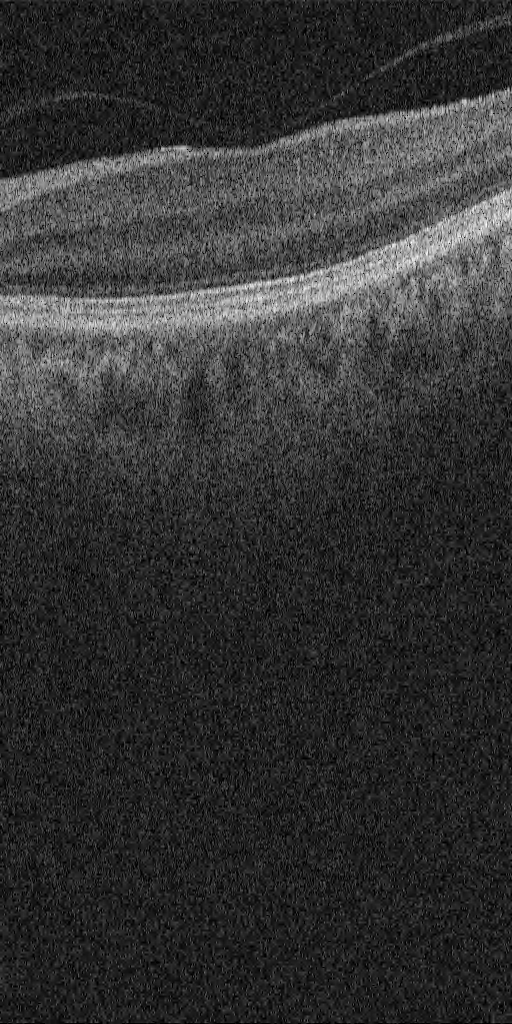
\includegraphics[scale=0.15]{normal_case.png}}\hfill
\subfigure[\ac{dme}-cyst]{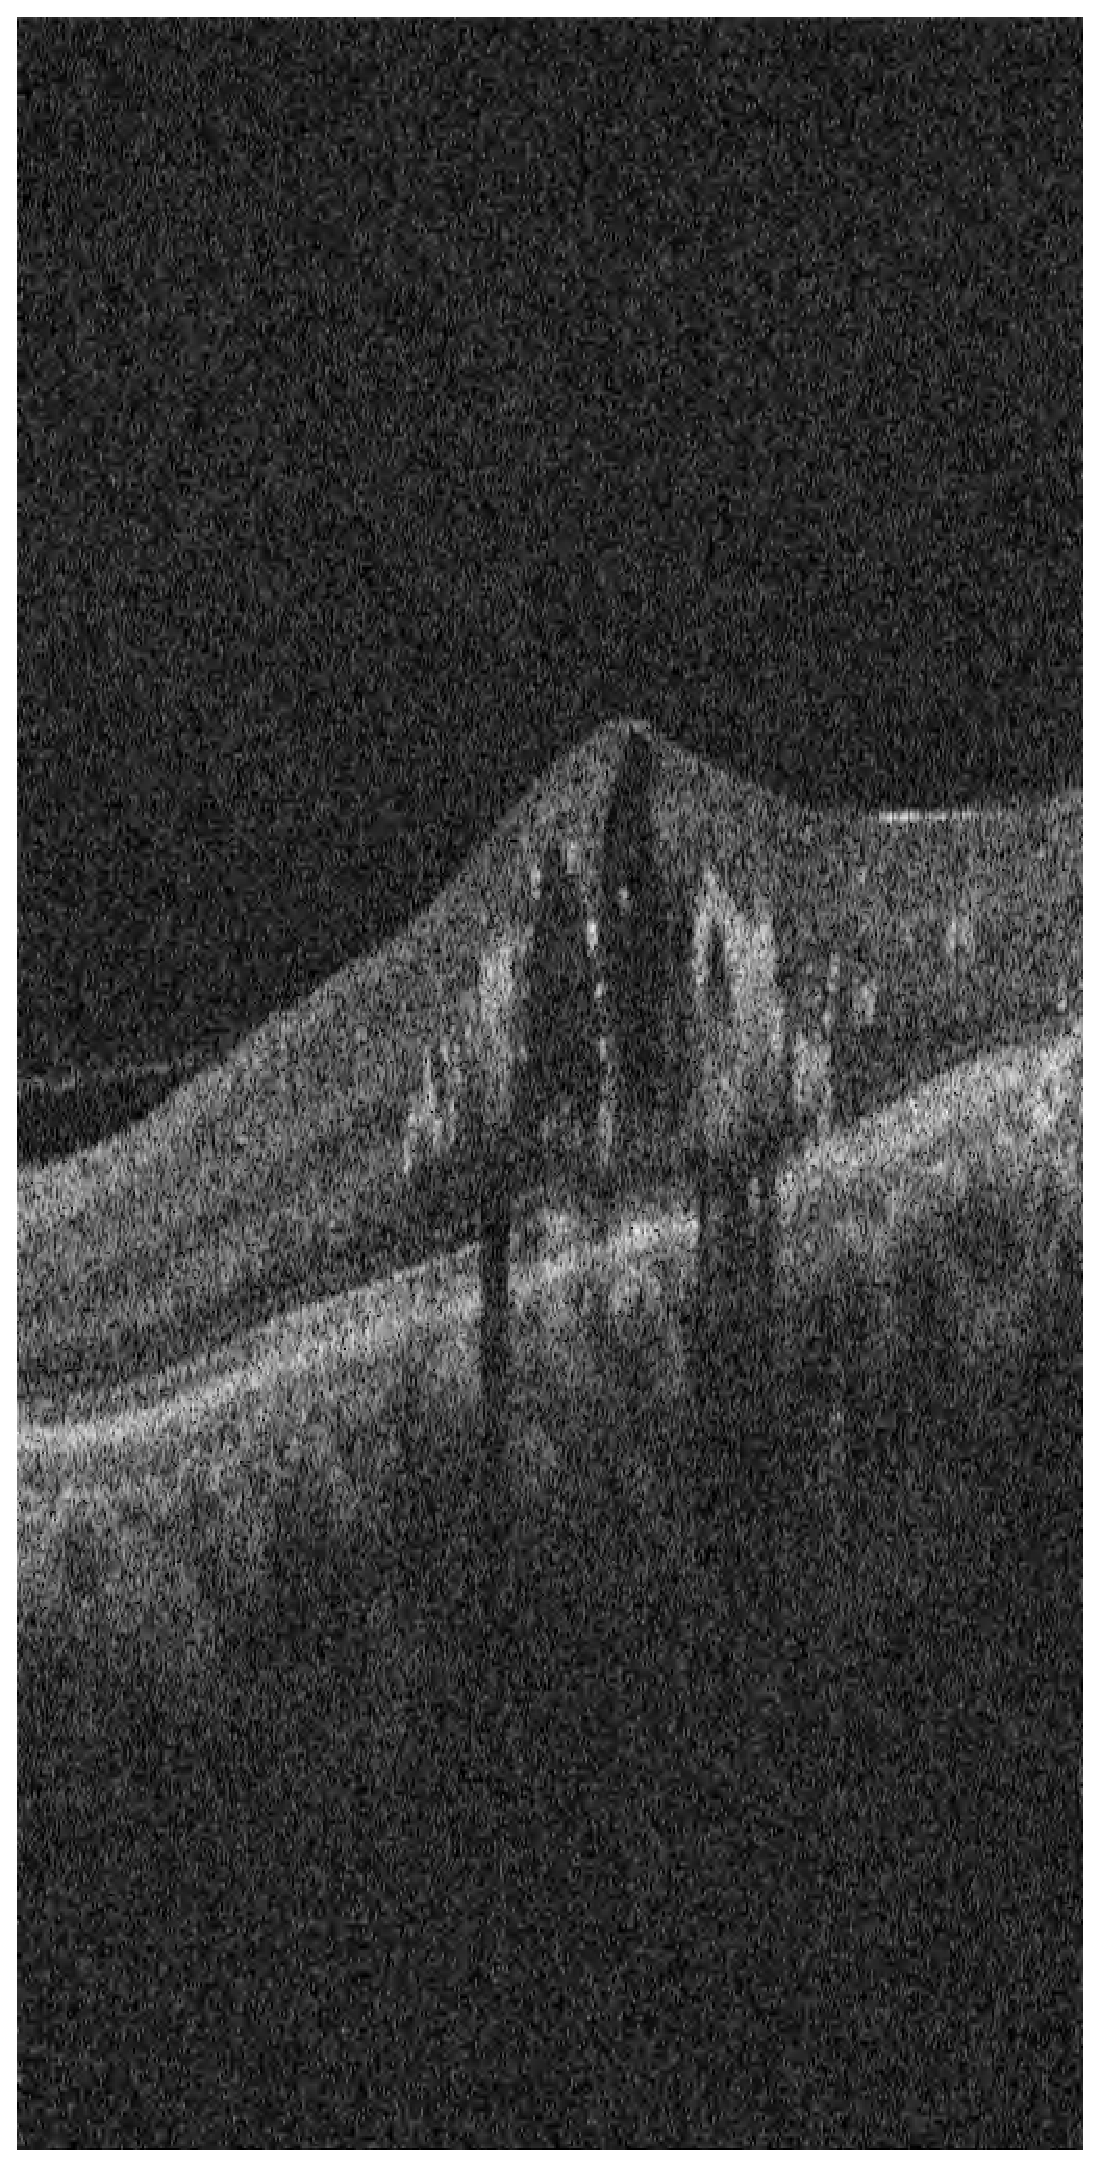
\includegraphics[scale=0.15]{dme_cyst}}\hfill
\subfigure[\ac{dme}-exudate]{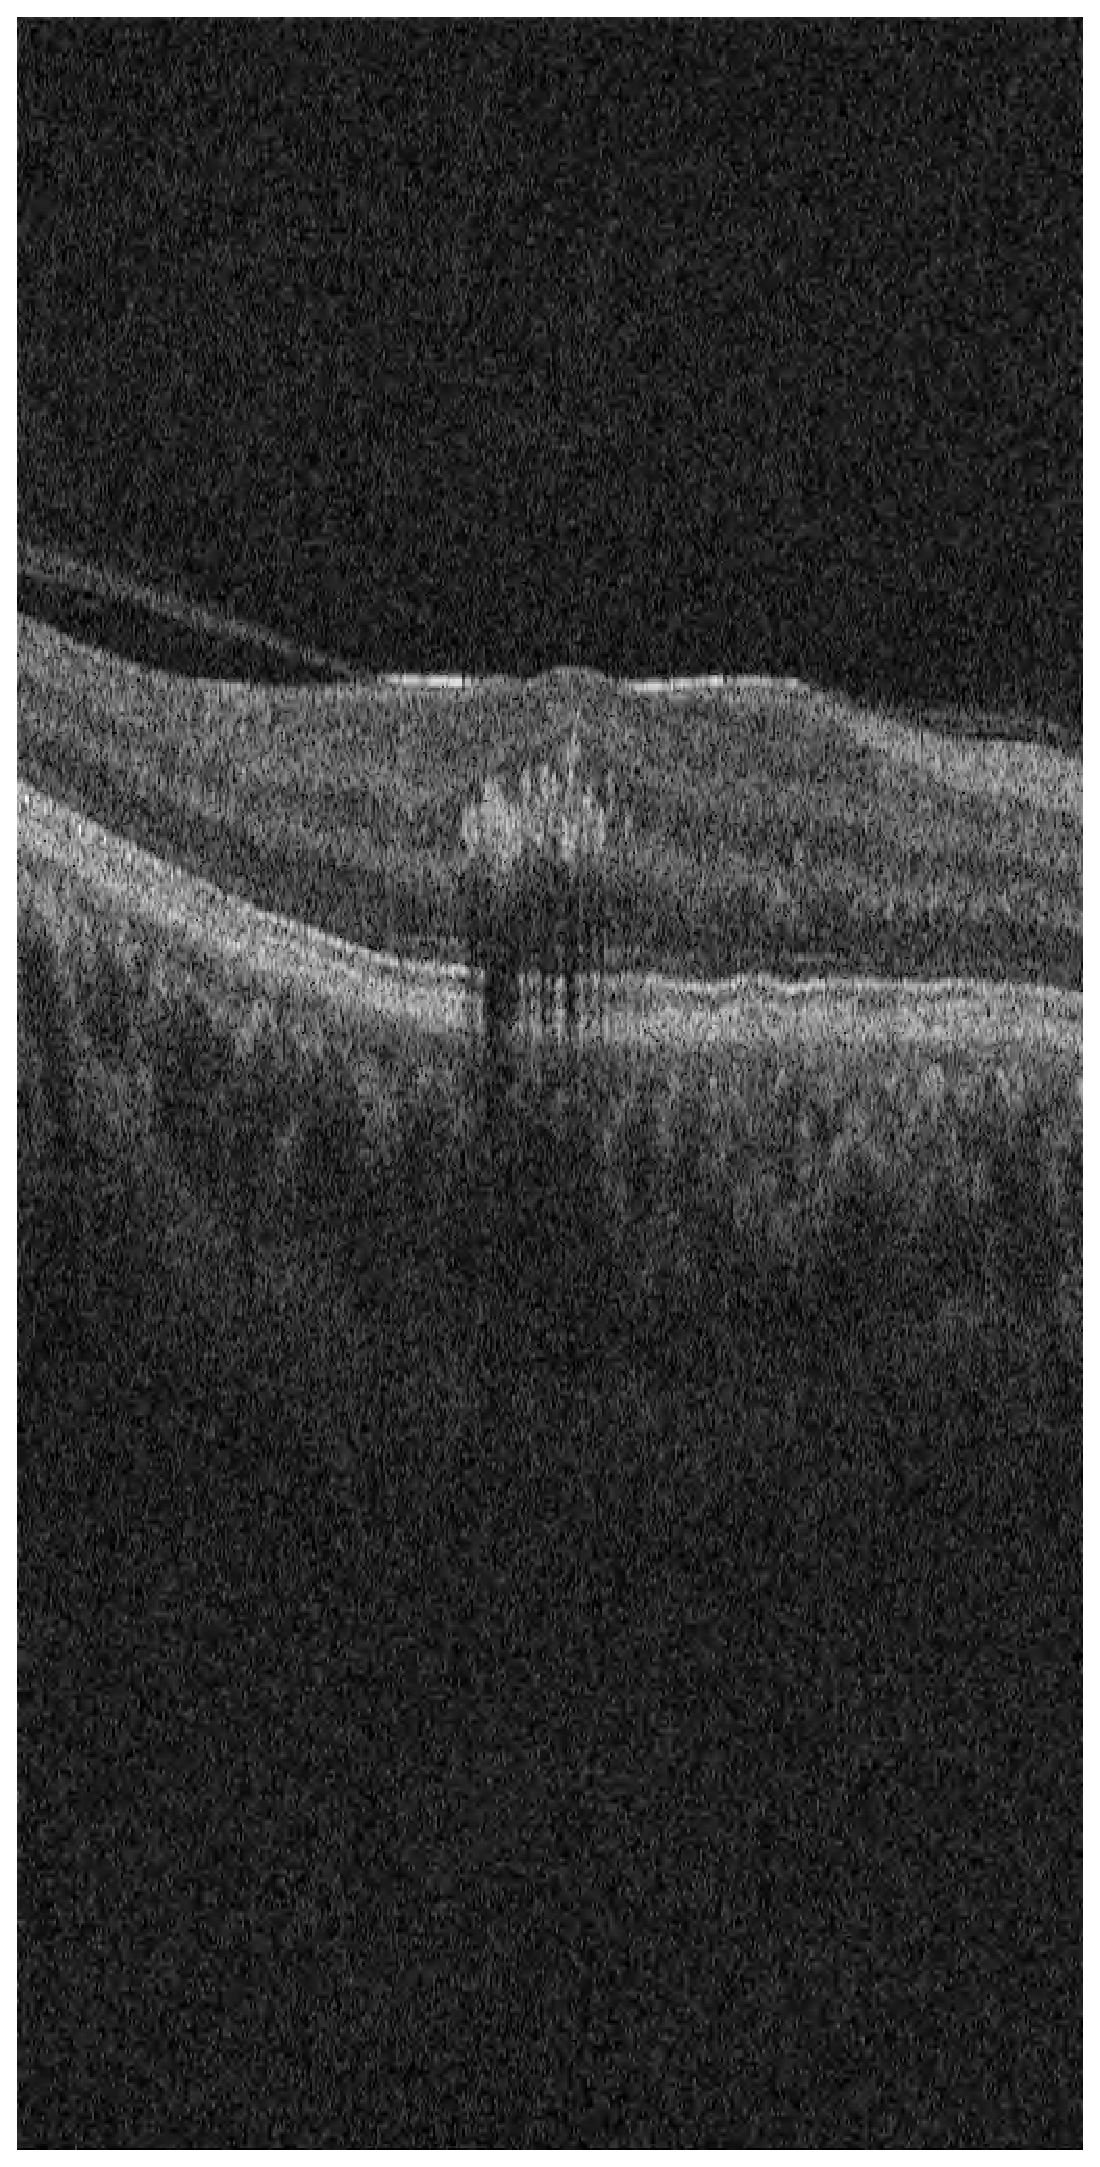
\includegraphics[scale=0.15]{dme_exudate}}
\hspace*{\fill}
\end{center}
\caption{ Example of \ac{sdoct} images for normal (a) and \ac{dme} patients (b)-(c) with cyst and exudate, respectively.}
\label{fig:dme-normal}
\end{figure}
Many of the previous works on \ac{oct} image analysis have focused on the problem of retinal layers segmentation, which is a necessary step for retinal thickness measurements~\cite{Chiu2010,Kafieh2013}.
However, few have addressed the specific problem of \ac{dme} and its associated features detection from \ac{oct} images.

A summary of the existing work can be found in Table~\ref{tab:survey-tab}.
Srinivasan\,\textit{et al.}~\cite{Srinivasan2014} proposed a classification method to distinguish \ac{dme}, \ac{amd} and normal \ac{sdoct} volumes.
The \ac{oct} images are pre-processed by reducing the speckle noise by enhancing the sparsity in a transform-domain and flattening the retinal curvature to reduce the inter-patient variations.
Then, \ac{hog} are extracted for each slice of a volume and a linear \ac{svm} is used for classification.
On a dataset of 45 patients equally subdivided into the three aforementioned classes, this method leads to a correct classification rate of $100 \%$, $100 \%$ and $86.67 \%$ for normal, \ac{dme} and \ac{amd} patients, respectively.
The images that have been used in their paper, are publicly available but are already preprocessed (i.e., denoised), have different sizes for the \ac{oct} volumes, do not offer a huge variability in term of \ac{dme} lesions, and some of them, without specifying which, have been excluded for the training phase; all these reasons prevent us from using this dataset to benchmark our work. 

Venhuizen\,\textit{et al.} proposed a method for \ac{oct} images classification using the \ac{bow} models~\cite{Venhuizen2015}.
The method starts with the detection and selection of keypoints in each individual B-scan, by keeping the most salient points corresponding to the top $3 \%$ of the vertical gradient values. Then, a texton of size $9 \times 9$ pixels is extracted around each keypoint, and \ac{pca} is applied to reduce the dimension of every texton to get a feature vector of size $9$.
All extracted feature vectors are used to create a codebook using \textit{k}-means clustering.
Then, each \ac{oct} volume is represented in terms of this codebook and is characterized as a histogram that captures the codebook occurrences.
These histograms are used as feature vector to train a \ac{rf} with a maximum of $100$ trees.
The method was used to classify \ac{oct} volumes between \ac{amd} and normal cases and achieved an \ac{auc} of $0.984$ with a dataset of $384$ \ac{oct} volumes.

Liu\,\textit{et al.} proposed a methodology for detecting macular pathology in \ac{oct} images using \ac{lbp} and gradient information as attributes~\cite{Liu2011}.
The method starts by aligning and flattening the images and creating a $3$-level multi-scale spatial pyramid.
The edge and \ac{lbp} histograms are then extracted from each block of every level of the pyramid.
%is created and edge and \ac{lbp} histograms are extracted in each block at every level of the pyramid.
All the obtained histograms are concatenated into a global descriptor whose dimensions are reduced using \ac{pca}.
Finally a \ac{svm} with an \ac{rbf} kernel is used as classifier.
The method achieved good results in detection \ac{oct} scan containing different pathology such as \ac{dme} or \ac{amd}, with an \ac{auc} of $0.93$ using a dataset of $326$ \ac{oct} scans.

{\color{red}Lemaitre~\emph{et al.}~\cite{Lemaintre2015miccaiOCT} proposed to use 2D and 3D \ac{lbp} features extracted from denoised volumes and dictionary learning using the \ac{bow} models~\cite{Sivic2003}.
In the proposed method all the dictionaries are learned with same size of ``visual words'' ($k = 32$) and final descriptors are classified using \ac{rf} classifier.
%The proposed method by Lemaitre~\emph{et al.}~\cite{Lemaintre2015miccaiOCT} is based on \ac{lbp} features to describe the texture of \ac{oct} images and dictionary learning using the \ac{bow} models~\cite{Sivic2003}.
The proposed method of this study is an extension of our previous work~\cite{Lemaintre2015miccaiOCT}\footnote{The Document source available on Github~\cite{Lemaitre2015}}.
In this research beside the comparison of 2D and 3D features and global and local mapping, we also compare the effects of common pre-processing steps for OCT data (i.e., aligning, flattening beside denoising), study the optimal configuration regarding the \ac{bow} approach and finally performance of different base classifiers.}
 
The proposed method, which is an extension of our previous work~\cite{Lemaintre2015miccaiOCT}\footnote{The Document source available on Github~\cite{Lemaitre2015}}, is based on \ac{lbp} features to describe the texture of \ac{oct} images and dictionary learning using the \ac{bow} models~\cite{Sivic2003}. 
We propose to extract 2D and 3D \ac{lbp} features from \ac{oct} images and volumes, respectively. 
The \ac{lbp} descriptors are further extracted from the entire sample or local patches within individual samples. 
In this research beside the comparison of 2D and 3D features, we also compare the effects of common pre-processing steps for OCT data (i.e., noise removing, aligning, flattening), study the optimal configuration regarding the \ac{bow} approach in conjunction with different base classifiers.
 
This paper is organized as follows: the proposed framework is explained in Sect.\,\ref{sec:method}, the experiments are presented in Sect.\,\ref{sec:exp}, while the results are discussed in Sect.\,\ref{sec:res-dis}.
{\color{red}while the experiments and results are discussed through Sect.\,\ref{sec:exp} and Sect.\,\ref{sec:res-dis}.}
Finally, the conclusion and avenue for future directions are drawn in Sect.\,\ref{sec:con}.

%----------

%%% Local Variables:
%%% TeX-master: "../../main.tex"
%%% TeX-master: "../../main.tex"
%%% End:
